\documentclass[aspectratio=169]{beamer}

% Theme and Color Setup
\usetheme{Madrid}
\usecolortheme{whale}
\useinnertheme{rectangles}
\useoutertheme{miniframes}

% Additional Packages
\usepackage[utf8]{inputenc}
\usepackage[T1]{fontenc}
\usepackage{graphicx}
\usepackage{booktabs}
\usepackage{listings}
\usepackage{amsmath}
\usepackage{amssymb}
\usepackage{xcolor}
\usepackage{tikz}
\usepackage{pgfplots}
\pgfplotsset{compat=1.18}
\usetikzlibrary{positioning}
\usepackage{hyperref}

% Custom Colors
\definecolor{myblue}{RGB}{31, 73, 125}
\definecolor{mygray}{RGB}{100, 100, 100}
\definecolor{mygreen}{RGB}{0, 128, 0}
\definecolor{myorange}{RGB}{230, 126, 34}
\definecolor{mycodebackground}{RGB}{245, 245, 245}

% Set Theme Colors
\setbeamercolor{structure}{fg=myblue}
\setbeamercolor{frametitle}{fg=white, bg=myblue}
\setbeamercolor{title}{fg=myblue}
\setbeamercolor{section in toc}{fg=myblue}
\setbeamercolor{item projected}{fg=white, bg=myblue}
\setbeamercolor{block title}{bg=myblue!20, fg=myblue}
\setbeamercolor{block body}{bg=myblue!10}
\setbeamercolor{alerted text}{fg=myorange}

% Set Fonts
\setbeamerfont{title}{size=\Large, series=\bfseries}
\setbeamerfont{frametitle}{size=\large, series=\bfseries}
\setbeamerfont{caption}{size=\small}
\setbeamerfont{footnote}{size=\tiny}

% Custom Commands
\newcommand{\hilight}[1]{\colorbox{myorange!30}{#1}}
\newcommand{\concept}[1]{\textcolor{myblue}{\textbf{#1}}}
\newcommand{\separator}{\begin{center}\rule{0.5\linewidth}{0.5pt}\end{center}}

% Title Page Information
\title[Week 4: Data Ingestion and Storage]{Week 4: Data Ingestion and Storage}
\author[J. Smith]{John Smith, Ph.D.}
\institute[University Name]{Department of Computer Science\\ University Name}
\date{\today}

% Document Start
\begin{document}

\frame{\titlepage}

\begin{frame}[fragile]
    \frametitle{Introduction to Data Ingestion and Storage}
    \begin{block}{Key Concepts}
        \begin{enumerate}
            \item \textbf{Data Ingestion}: The process of collecting and importing data for immediate use or storage in a database. It enables organizations to leverage real-time and historical data for analytics.
            \item \textbf{Data Storage}: Effective storage solutions are crucial for future data retrieval and processing, influencing analysis and decision-making processes.
        \end{enumerate}
    \end{block}
\end{frame}

\begin{frame}[fragile]
    \frametitle{Importance of Data Ingestion and Storage}
    \begin{itemize}
        \item \textbf{Scalability}:
            \begin{itemize}
                \item Data volumes grow exponentially; efficient systems can scale to handle large influxes.
                \item Example: Apache Kafka offers scalable data streaming capabilities.
            \end{itemize}
        
        \item \textbf{Speed}:
            \begin{itemize}
                \item Instant access enables rapid analytical response times.
                \item Example: NoSQL databases like MongoDB allow for real-time queries.
            \end{itemize}
        
        \item \textbf{Data Quality \& Integrity}:
            \begin{itemize}
                \item Quality ingestion processes ensure data integrity and reduce errors.
                \item Automated pipelines can verify data formats to prevent data corruption.
            \end{itemize}
    \end{itemize}
\end{frame}

\begin{frame}[fragile]
    \frametitle{Examples of Data Ingestion and Storage Solutions}
    \begin{block}{Ingestion Methods}
        \begin{itemize}
            \item \textbf{Batch Processing}:
                \begin{itemize}
                    \item Tools like Apache NiFi facilitate periodic batch ingestion of datasets.
                    \item \textit{Example}: Daily sales data loading from CSV files into a data warehouse.
                \end{itemize}
            
            \item \textbf{Real-time Processing}:
                \begin{itemize}
                    \item Apache Kafka streams data in real-time from multiple sources.
                    \item \textit{Example}: Capturing user interactions on a website for immediate analysis.
                \end{itemize}
        \end{itemize}
    \end{block}

    \begin{block}{Storage Solutions}
        \begin{itemize}
            \item \textbf{Relational Databases}: MySQL, PostgreSQL (structured data with fixed schemas).
            \item \textbf{NoSQL Databases}: Cassandra, MongoDB (unstructured data with flexible schema designs).
            \item \textbf{Data Lakes}: AWS S3, Azure Data Lake (storage for raw data, suitable for big data analysis).
        \end{itemize}
    \end{block}
\end{frame}

\begin{frame}[fragile]
    \frametitle{Introduction to ETL}
    \begin{block}{What is ETL?}
        ETL stands for Extract, Transform, Load. It is a data integration process involving:
        \begin{enumerate}
            \item Extracting data from various sources
            \item Transforming the data into a suitable format for analysis
            \item Loading the transformed data into a data warehouse or other storage solutions
        \end{enumerate}
    \end{block}
\end{frame}

\begin{frame}[fragile]
    \frametitle{Importance of ETL in Data Workflows}
    \begin{itemize}
        \item Integration of Data from Multiple Sources: Combines data from different systems for comprehensive analysis.
        \item Improved Data Quality: Cleans and reconciles discrepancies to improve data quality prior to analysis.
        \item Performance Optimization: Optimizes ETL processes to enhance efficiency in data ingestion and processing.
    \end{itemize}
\end{frame}

\begin{frame}[fragile]
    \frametitle{Breakdown of the ETL Process}
    \begin{block}{1. Extract}
        \begin{itemize}
            \item Definition: Pulling data from systems like databases, web services, files.
            \item Example: Extracting customer, sales, and product data from relevant platforms.
            \item Common Techniques:
                \begin{itemize}
                    \item Full extraction
                    \item Incremental extraction
                    \item Using API calls for real-time data access
                \end{itemize}
        \end{itemize}
    \end{block}
    
    \begin{block}{2. Transform}
        \begin{itemize}
            \item Definition: Operations to convert data into the required format.
            \item Examples:
                \begin{itemize}
                    \item Data cleansing, aggregation, type conversion
                \end{itemize}
            \item Key Transform Functions:
                \begin{lstlisting}[language=SQL]
SELECT * FROM Customers JOIN Orders ON Customers.ID = Orders.CustomerID;
                \end{lstlisting}
        \end{itemize}
    \end{block}
\end{frame}

\begin{frame}[fragile]
    \frametitle{ETL Process Continued}
    \begin{block}{3. Load}
        \begin{itemize}
            \item Definition: Storing the transformed data into a target system.
            \item Loading Strategies:
                \begin{itemize}
                    \item Full Load: Load entire dataset.
                    \item Incremental Load: Load only new or updated records.
                \end{itemize}
            \item Example: Loading monthly sales reports into a data warehouse.
        \end{itemize}
    \end{block}
\end{frame}

\begin{frame}[fragile]
    \frametitle{Key Points to Remember}
    \begin{itemize}
        \item ETL is essential for effective data warehousing and analytics.
        \item The extraction process is fundamental to data gathering.
        \item Transformations enhance data accuracy and usability.
        \item Efficient loading strategies improve performance.
    \end{itemize}
\end{frame}

\begin{frame}[fragile]
    \frametitle{Simple ETL Workflow Diagram}
    \centering
    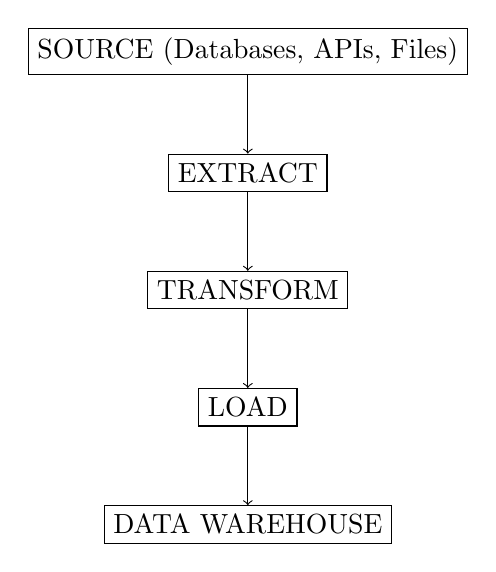
\begin{tikzpicture}
        \node (source) [draw, rectangle] {SOURCE (Databases, APIs, Files)};
        \node (extract) [draw, rectangle, below=of source] {EXTRACT};
        \node (transform) [draw, rectangle, below=of extract] {TRANSFORM};
        \node (load) [draw, rectangle, below=of transform] {LOAD};
        \node (warehouse) [draw, rectangle, below=of load] {DATA WAREHOUSE};

        \draw[->] (source) -- (extract);
        \draw[->] (extract) -- (transform);
        \draw[->] (transform) -- (load);
        \draw[->] (load) -- (warehouse);
    \end{tikzpicture}
\end{frame}

\begin{frame}[fragile]
    \frametitle{Conclusion}
    \begin{block}{Understanding ETL}
        ETL processes are foundational for data management and analytics, enabling effective decision-making. Understanding ETL is crucial for anyone involved in data workflows as it significantly impacts data quality and reporting outcomes.
    \end{block}
\end{frame}

\begin{frame}[fragile]
  \frametitle{Data Sources for Ingestion}
  \begin{block}{Overview of Data Sources}
    Data ingestion is a critical step in the ETL (Extract, Transform, Load) process. Understanding the types of data encountered is essential for effective data management. Data sources can be categorized into three types:
    \begin{itemize}
      \item \textbf{Structured Data}
      \item \textbf{Semi-structured Data}
      \item \textbf{Unstructured Data}
    \end{itemize}
  \end{block}
\end{frame}

\begin{frame}[fragile]
  \frametitle{1. Structured Data}
  \textbf{Definition:} Data that adheres to a pre-defined data model, organized in tables with fixed columns and rows.

  \begin{itemize}
    \item \textbf{Characteristics:}
      \begin{itemize}
        \item Easily searchable using standard SQL queries
        \item Schema-driven, with data format defined beforehand
      \end{itemize}
    
    \item \textbf{Examples:}
      \begin{itemize}
        \item Relational databases (e.g., MySQL, Oracle)
        \item Spreadsheets (e.g., Excel files)
      \end{itemize}
    
    \item \textbf{Use Cases:}
      \begin{itemize}
        \item Financial reporting
        \item Inventory management
        \item Customer databases
      \end{itemize}
  \end{itemize}
\end{frame}

\begin{frame}[fragile]
  \frametitle{2. Semi-structured Data}
  \textbf{Definition:} Data that does not reside in a relational database but has some organizational properties.

  \begin{itemize}
    \item \textbf{Characteristics:}
      \begin{itemize}
        \item Contains tags or markers for element separation (e.g., JSON, XML)
        \item Flexible schema that can evolve over time
      \end{itemize}
    
    \item \textbf{Examples:}
      \begin{itemize}
        \item JSON files from web APIs
        \item XML documents
      \end{itemize}
    
    \item \textbf{Use Cases:}
      \begin{itemize}
        \item Data from social media platforms
        \item Log files
        \item Configuration files
      \end{itemize}
  \end{itemize}
\end{frame}

\begin{frame}[fragile]
  \frametitle{3. Unstructured Data}
  \textbf{Definition:} Data that lacks a predefined data model and is often not easily searchable.

  \begin{itemize}
    \item \textbf{Characteristics:}
      \begin{itemize}
        \item No uniform format; highly diverse
        \item Requires advanced processing techniques for analysis (e.g., Natural Language Processing)
      \end{itemize}
    
    \item \textbf{Examples:}
      \begin{itemize}
        \item Text documents (e.g., PDFs, Word files)
        \item Multimedia files (e.g., images, audio, and video)
      \end{itemize}
    
    \item \textbf{Use Cases:}
      \begin{itemize}
        \item Customer feedback analysis
        \item Sentiment analysis
        \item Machine learning applications
      \end{itemize}
  \end{itemize}
\end{frame}

\begin{frame}[fragile]
  \frametitle{Key Points and Conclusion}
  \begin{itemize}
    \item Different data types require different ingestion and processing techniques.
    \item Understanding the nature of data is crucial for selecting an appropriate data storage solution.
    \item Combining and analyzing structured, semi-structured, and unstructured data can provide valuable insights for business intelligence.
  \end{itemize}

  \textbf{Conclusion:} Identifying the type of data source is key to effective data ingestion in ETL workflows. An iterative approach fosters comprehensive analytical outcomes, enhancing overall insight generation.
\end{frame}

\begin{frame}[fragile]
  \frametitle{Data Ingestion Techniques}
  \begin{block}{Introduction to Data Ingestion}
    Data ingestion is the process of obtaining and importing data for immediate use or storage in a database. 
    It's essential to the data pipeline and lays the foundation for:
    \begin{itemize}
      \item Data analysis
      \item Data transformation
      \item Data visualization
    \end{itemize}
  \end{block}
\end{frame}

\begin{frame}[fragile]
  \frametitle{Common Data Ingestion Techniques}
  \begin{enumerate}
    \item \textbf{Batch Processing}
    \item \textbf{Real-Time Streaming}
  \end{enumerate}
\end{frame}

\begin{frame}[fragile]
  \frametitle{Batch Processing}
  \begin{block}{Overview}
    Batch processing involves collecting and storing data over a set period before processing it as a single unit (batch).
  \end{block}
  \begin{itemize}
    \item \textbf{Examples:}
    \begin{itemize}
      \item Financial transactions: End-of-day transaction reports
      \item System log files: Analysis of collected logs during off-peak hours
    \end{itemize}
    \item \textbf{Pros:}
    \begin{itemize}
      \item Efficient with large volumes of data
      \item Reduces system load during busy times
    \end{itemize}
    \item \textbf{Cons:}
    \begin{itemize}
      \item Data latency; insights are not real-time
      \item Requires periodic execution, missing immediate insights
    \end{itemize}
  \end{itemize}
\end{frame}

\begin{frame}[fragile]
  \frametitle{Real-Time Streaming}
  \begin{block}{Overview}
    Real-time streaming processes data continuously as it is generated, ideal for applications requiring immediate insights.
  \end{block}
  \begin{itemize}
    \item \textbf{Examples:}
    \begin{itemize}
      \item Social media feeds: Adjust marketing strategies in real time
      \item Financial trading systems: Instantaneous decision making based on stock fluctuations
    \end{itemize}
    \item \textbf{Pros:}
    \begin{itemize}
      \item Immediate insights and responsive actions
      \item Suitable for time-sensitive applications like fraud detection
    \end{itemize}
    \item \textbf{Cons:}
    \begin{itemize}
      \item More complex infrastructure requirements
      \item Higher resource consumption due to continuous processing
    \end{itemize}
  \end{itemize}
\end{frame}

\begin{frame}[fragile]
  \frametitle{Key Points to Emphasize}
  \begin{itemize}
    \item \textbf{Batch vs. Real-Time:} Understand trade-offs between data latency and processing needs.
    \item \textbf{Application Relevance:} Choose a method based on use cases—for example:
    \begin{itemize}
      \item Retail company: Batch processing for sales reports
      \item Cybersecurity firm: Real-time streaming for threat detection
    \end{itemize}
  \end{itemize}
\end{frame}

\begin{frame}[fragile]
  \frametitle{Conclusion}
  \begin{block}{Conclusion}
    Data ingestion techniques are pivotal in how we interact with data. Choosing between batch processing and real-time streaming depends on specific data strategy needs. 
  \end{block}
  \begin{itemize}
    \item Batch processing offers efficiency.
    \item Real-time streaming provides immediacy.
  \end{itemize}
\end{frame}

\begin{frame}[fragile]
  \frametitle{Visuals Suggestion}
  \begin{itemize}
    \item \textbf{Diagram of Data Ingestion Flow:} Illustrate data entering the pipeline through either method and flowing into storage or analytics units.
    \item \textbf{Comparison Table:} Comparing batch processing and real-time streaming based on:
    \begin{itemize}
      \item Speed
      \item Complexity
      \item Resource usage
    \end{itemize}
  \end{itemize}
\end{frame}

\begin{frame}[fragile]
    \frametitle{Transforming Data - Overview}
    \begin{block}{Overview of Transformation Processes}
        Data transformation is a critical step in the data pipeline. 
        It involves the modification of data to make it suitable for analysis, storage, and further processing. Key transformation processes include:
    \end{block}
    
    \begin{itemize}
        \item Data Cleaning
        \item Normalization
        \item Aggregation
    \end{itemize}
\end{frame}

\begin{frame}[fragile]
    \frametitle{Transforming Data - Data Cleaning}
    \begin{block}{Data Cleaning}
        \begin{itemize}
            \item \textbf{Definition}: Identifying and correcting errors or inconsistencies in data to improve its quality.
            \item \textbf{Common Tasks}:
            \begin{enumerate}
                \item Removing Duplicates
                \item Handling Missing Values
                \begin{itemize}
                    \item Imputation
                    \item Removal
                \end{itemize}
                \item Correcting Inaccuracies
            \end{enumerate}
            \item \textbf{Example}: Standardizing entries (e.g., 'John D.' vs 'Jon Doe').
        \end{itemize}
    \end{block}
\end{frame}

\begin{frame}[fragile]
    \frametitle{Transforming Data - Normalization and Aggregation}
    \begin{block}{Normalization}
        \begin{itemize}
            \item \textbf{Definition}: Scaling data into a specific range, typically [0, 1].
            \item \textbf{Techniques}:
            \begin{itemize}
                \item Min-Max Scaling: 
                \[
                X' = \frac{X - X_{min}}{X_{max} - X_{min}}
                \]
                \item Z-Score Normalization:
                \[
                Z = \frac{(X - \mu)}{\sigma}
                \]
            \end{itemize}
            \item \textbf{Example}: Normalizing test scores and ages for model inputs.
        \end{itemize}
    \end{block}

    \begin{block}{Aggregation}
        \begin{itemize}
            \item \textbf{Definition}: Combining multiple data points into a single summary operation.
            \item \textbf{Common Functions}:
            \begin{itemize}
                \item Sum
                \item Average
                \item Count
            \end{itemize}
            \item \textbf{Example}: Total revenue from customer transactions.
        \end{itemize}
    \end{block}
\end{frame}

\begin{frame}[fragile]
    \frametitle{Transforming Data - Key Points and Visual}
    \begin{block}{Key Points to Emphasize}
        \begin{itemize}
            \item Data Transformation is Essential
            \item Quality Matters
            \item Scale and Summarize
        \end{itemize}
    \end{block}

    \begin{block}{Visual Illustration}
        Consider adding a flowchart:
        \[
        \text{Raw Data} \rightarrow \text{Data Cleaning} \rightarrow \text{Normalized Data} \rightarrow \text{Aggregated Data} \rightarrow \text{Insights}
        \end{block}
\end{frame}

\begin{frame}[fragile]
    \frametitle{Loading Data into Storage Solutions - Overview}
    \begin{block}{Introduction to Storage Solutions}
        Selecting the right storage solution is essential for efficiently handling large volumes of structured and unstructured data.
    \end{block}
    \begin{itemize}
        \item 1. \textbf{Data Warehouses}
        \item 2. \textbf{Data Lakes}
    \end{itemize}
\end{frame}

\begin{frame}[fragile]
    \frametitle{Loading Data into Storage Solutions - Data Warehouses}
    \begin{block}{Definition}
        A data warehouse is a centralized repository designed for reporting and data analysis, primarily used for structured data.
    \end{block}
    \begin{itemize}
        \item \textbf{Characteristics:}
        \begin{itemize}
            \item Optimized for complex queries and analytics.
            \item Schema-on-write: Data is processed and organized before being stored.
        \end{itemize}
        \item \textbf{Loading Process:}
        \begin{itemize}
            \item Extract, Transform, Load (ETL): Data is extracted from various sources, transformed, and loaded into the warehouse.
        \end{itemize}
        \item \textbf{Example:}
        A retail company gathers transaction data daily; this data undergoes ETL processes to analyze sales trends and inventory status.
    \end{itemize}
\end{frame}

\begin{frame}[fragile]
    \frametitle{Loading Data into Storage Solutions - Data Lakes}
    \begin{block}{Definition}
        A data lake is a storage repository that holds vast amounts of raw data in its native format until it is needed for analysis.
    \end{block}
    \begin{itemize}
        \item \textbf{Characteristics:}
        \begin{itemize}
            \item Can store structured, semi-structured, and unstructured data.
            \item Schema-on-read: Data is organized only when it is read for analysis.
        \end{itemize}
        \item \textbf{Loading Process:}
        \begin{itemize}
            \item Extract, Load: Data is extracted from sources and loaded directly into the lake without transformation.
        \end{itemize}
        \item \textbf{Example:}
        A social media platform stores user-generated content (posts, comments, images) in a data lake for future analysis.
    \end{itemize}
\end{frame}

\begin{frame}[fragile]
    \frametitle{Loading Data into Storage Solutions - Key Points}
    \begin{itemize}
        \item \textbf{Choosing the Right Solution:}
        \begin{itemize}
            \item Data warehouses are ideal for analytical tasks requiring structured data.
            \item Data lakes offer flexibility and the ability to process varied types of data.
        \end{itemize}
        \item \textbf{Loading Methodologies:}
        \begin{itemize}
            \item ETL is critical for data warehouses to ensure data quality.
            \item Direct loading into data lakes supports big data initiatives.
        \end{itemize}
    \end{itemize}
\end{frame}

\begin{frame}[fragile]
    \frametitle{Loading Data into Storage Solutions - Summary}
    Understanding the differences between data warehouses and data lakes, as well as their respective loading processes, is crucial for effectively managing and analyzing data.
    \begin{block}{Next Steps}
        We will discuss challenges associated with data ingestion and storage, such as data quality and latency.
    \end{block}
\end{frame}

\begin{frame}[fragile]
    \frametitle{Challenges in Data Ingestion and Storage - Overview}
    \begin{itemize}
        \item Data ingestion and storage are critical in data architecture.
        \item Organizations face challenges that affect data-driven decision-making.
        \item This presentation highlights:
        \begin{itemize}
            \item Data Quality
            \item Latency
            \item Scalability
            \item Data Integration
        \end{itemize}
    \end{itemize}
\end{frame}

\begin{frame}[fragile]
    \frametitle{Challenges in Data Ingestion and Storage - Data Quality}
    \begin{block}{Data Quality}
        \textbf{Definition:} Accuracy, completeness, and reliability of data.\\
        Poor data quality can lead to faulty insights and decisions.
    \end{block}
    \begin{exampleblock}{Illustration Example}
        \textbf{Scenario:} Retail company collecting customer data.
        \begin{itemize}
            \item Challenge: Inconsistencies in names (e.g., "Jonathan" vs. "Jon") lead to duplicates.
        \end{itemize}
    \end{exampleblock}
    \begin{itemize}
        \item \textbf{Importance:} Affects business intelligence outputs.
        \item \textbf{Common Issues:} Missing values, duplicates, outdated data.
    \end{itemize}
\end{frame}

\begin{frame}[fragile]
    \frametitle{Challenges in Data Ingestion and Storage - Latency, Scalability, and Integration}
    \begin{block}{Latency}
        \textbf{Definition:} Delay between data generation and availability for analysis.\\
        High latency can impede real-time analytics.
    \end{block}
    \begin{exampleblock}{Illustration Example}
        \textbf{Scenario:} Financial firm needing real-time data for trading.\\
        Challenge: Delayed ingestion may result in lost opportunities.
    \end{exampleblock}
    
    \begin{block}{Scalability}
        \textbf{Definition:} Ability to handle increasing data efficiently without performance loss.\\
    \end{block}
    \begin{exampleblock}{Illustration Example}
        \textbf{Scenario:} E-commerce platform during flash sales.\\
        Challenge: Traditional solutions may fail to scale, causing crashes.
    \end{exampleblock}
    
    \begin{block}{Data Integration}
        \textbf{Definition:} Consolidating data from various sources into a unified view.\\
        \textbf{Importance:} Integrated data provides better insights.
    \end{block}
    \begin{exampleblock}{Illustration Example}
        \textbf{Scenario:} Healthcare provider with data from multiple departments.\\
        Challenge: Disparate systems cause data silos, complicating analytics.
    \end{exampleblock}
\end{frame}

\begin{frame}[fragile]
    \frametitle{Conclusion and Next Steps}
    \begin{itemize}
        \item Addressing challenges in ingestion and storage enhances data effectiveness.
        \item Organizations should:
        \begin{itemize}
            \item Invest in robust systems for high data quality.
            \item Ensure low latency and scalable solutions.
            \item Implement effective data integration processes.
        \end{itemize}
        \item \textbf{Next Steps:} Upcoming slide explores key ETL technologies to mitigate challenges and improve data management strategies.
    \end{itemize}
\end{frame}

\begin{frame}[fragile]
    \frametitle{Key Technologies for ETL - Overview}
    \begin{block}{ETL Overview}
        ETL stands for \textbf{Extract, Transform, Load}. It is a crucial process in data integration involving:
        \begin{itemize}
            \item Extracting data from various sources
            \item Transforming it to fit operational needs
            \item Loading it into a destination database or data warehouse
        \end{itemize}
        The right ETL tool can significantly enhance efficiency and data quality.
    \end{block}
\end{frame}

\begin{frame}[fragile]
    \frametitle{Key Technologies for ETL - ETL Tools}
    \begin{block}{Major ETL Tools and Frameworks}
        \begin{enumerate}
            \item \textbf{Apache NiFi}
                \begin{itemize}
                    \item \textbf{Description}: An open-source tool that supports data flow automation.
                    \item \textbf{Key Features}:
                        \begin{itemize}
                            \item Flow-based programming model
                            \item Real-time data ingestion and monitoring
                            \item User-friendly web interface
                        \end{itemize}
                    \item \textbf{Example Use Case}: Automate log ingestion from servers for real-time monitoring.
                \end{itemize}
            \item \textbf{Talend}
                \begin{itemize}
                    \item \textbf{Description}: A widely used ETL tool offering both cloud and on-premises solutions.
                    \item \textbf{Key Features}:
                        \begin{itemize}
                            \item Open-source version with a wide range of connectors
                            \item Drag-and-drop interface for workflow design
                            \item Extensive transformation capabilities
                        \end{itemize}
                    \item \textbf{Example Use Case}: Extract and transform customer data from multiple CRM systems.
                \end{itemize}
            \item \textbf{Custom-built Solutions}
                \begin{itemize}
                    \item \textbf{Description}: Tailor-made systems designed to address specific ETL requirements.
                    \item \textbf{Key Features}:
                        \begin{itemize}
                            \item Complete flexibility for unique business needs
                            \item Can utilize programming languages (e.g., Python, Java)
                            \item Requires more development and maintenance resources
                        \end{itemize}
                    \item \textbf{Example Use Case}: A specialized process using Python to transform data from APIs.
                \end{itemize}
        \end{enumerate}
    \end{block}
\end{frame}

\begin{frame}[fragile]
    \frametitle{Key Technologies for ETL - Considerations}
    \begin{block}{Key Points to Emphasize}
        \begin{itemize}
            \item \textbf{Understanding Requirements}: Choice of tool depends on volume, complexity, budget, and ecosystem.
            \item \textbf{Scalability and Performance}: Opt for tools that can scale horizontally for growing data needs.
            \item \textbf{Compliance and Security}: Ensure adherence to data governance and security requirements.
            \item \textbf{Ease of Use}: User-friendly interfaces reduce the learning curve and speed up implementation.
        \end{itemize}
    \end{block}
    
    \begin{block}{Diagram: Data Flow}
        \centering
        \includegraphics[width=0.7\linewidth]{diagram.png}
        % The diagram can be included as an external image or drawn with TikZ
    \end{block}
    
    \begin{block}{Conclusion}
        By understanding and choosing the appropriate ETL tools, organizations can manage data workflows efficiently, ensuring high data quality and timely availability for analysis, which is critical in a machine learning context.
    \end{block}
\end{frame}

\begin{frame}[fragile]
    \frametitle{Cloud-based Data Storage Solutions - Overview}
    \begin{block}{Overview}
        In today's data-driven world, efficient data storage is crucial for managing vast volumes of data generated by businesses. Cloud storage solutions, such as AWS S3 (Amazon Simple Storage Service) and Google Cloud Storage, offer scalable options for data ingestion, allowing organizations to store, retrieve, and process large datasets efficiently.
    \end{block}
\end{frame}

\begin{frame}[fragile]
    \frametitle{Cloud-based Data Storage Solutions - Key Concepts}
    \begin{enumerate}
        \item \textbf{What is Cloud Storage?}
        \begin{itemize}
            \item Storage of data on remote servers accessed via the internet.
            \item Benefits include:
                \begin{itemize}
                    \item Scalability
                    \item Data security
                    \item Redundancy
                    \item Reduced IT management costs
                \end{itemize}
        \end{itemize}
        
        \item \textbf{Benefits of Cloud Storage for Data Ingestion:}
        \begin{itemize}
            \item \textbf{Scalability:} Increase storage easily without physical hardware.
            \item \textbf{Accessibility:} Access data from any location with internet connectivity.
            \item \textbf{Cost-Effective:} Pay only for what you use.
            \item \textbf{Durability and Availability:} High durability and quick access in services like AWS S3 and GCS.
        \end{itemize}
    \end{enumerate}
\end{frame}

\begin{frame}[fragile]
    \frametitle{Cloud-based Data Storage Solutions - AWS S3 vs Google Cloud Storage}
    \begin{block}{AWS S3}
        \begin{itemize}
            \item Highly scalable and reliable object storage service.
            \item \textbf{Key Features:}
            \begin{itemize}
                \item Bucket Creation
                \item Lifecycle Policies
                \item Access Control
            \end{itemize}
            \item \textbf{Use Case:} Media companies storing large files for streaming.
        \end{itemize}
    \end{block}

    \begin{block}{Google Cloud Storage}
        \begin{itemize}
            \item Unified object storage service for developers and enterprises.
            \item \textbf{Key Features:}
            \begin{itemize}
                \item Multi-Region Storage
                \item Class Storage Options
                \item Versioning Support
            \end{itemize}
            \item \textbf{Use Case:} Online retailers storing transaction data and product images.
        \end{itemize}
    \end{block}
\end{frame}

\begin{frame}[fragile]
    \frametitle{Cloud-based Data Storage Solutions - Comparison}
    \begin{table}[htbp]
        \centering
        \begin{tabular}{|l|c|c|}
            \hline
            \textbf{Feature} & \textbf{AWS S3} & \textbf{Google Cloud Storage} \\
            \hline
            Pricing Model & Pay-as-you-go & Pay-as-you-go \\
            Storage Classes & Multiple (Standard, Infrequent Access, Glacier) & Multiple (Standard, Nearline, Coldline, Archive) \\
            Data Access Methods & REST API, SDKs & JSON API, XML API, gcloud CLI \\
            Regional Availability & Global data centers & Global data centers \\
            Integration & Integrates with other AWS services & Integrates with the Google Cloud ecosystem \\
            \hline
        \end{tabular}
    \end{table}
\end{frame}

\begin{frame}[fragile]
    \frametitle{Cloud-based Data Storage Solutions - Key Takeaways}
    \begin{itemize}
        \item Cloud storage solutions like AWS S3 and Google Cloud Storage provide scalable, flexible, and cost-effective options for data ingestion.
        \item Selecting the right cloud storage service depends on specific business requirements, including data type, access patterns, and regulatory needs.
    \end{itemize}
\end{frame}

\begin{frame}[fragile]
    \frametitle{Case Studies: Successful Data Ingestion}
    \begin{block}{Introduction to Data Ingestion}
        \begin{itemize}
            \item \textbf{Definition}: The process of obtaining and importing data for immediate use or storage in a database.
            \item \textbf{Importance}: Consolidates data from various sources for analysis and decision-making.
        \end{itemize}
    \end{block}
\end{frame}

\begin{frame}[fragile]
    \frametitle{Importance of Successful Data Ingestion}
    \begin{itemize}
        \item Improved data accuracy and integrity.
        \item Enhanced performance for real-time analytics.
        \item Scalability to accommodate growing data volumes.
    \end{itemize}
\end{frame}

\begin{frame}[fragile]
    \frametitle{Case Study 1: Uber}
    \begin{block}{Context}
        Uber requires real-time data to track rides, driver availability, and demand.
    \end{block}
    \begin{block}{Ingestion Strategy}
        \begin{itemize}
            \item Custom-built data pipeline using Kafka (real-time streaming) and AWS S3 (scalable storage).
            \item Ingestion from various sources like mobile apps and GPS systems.
        \end{itemize}
    \end{block}
    \begin{block}{Outcome}
        \begin{itemize}
            \item Enhanced decision-making capabilities.
            \item Improved customer experience through predictive analytics for surge pricing.
        \end{itemize}
    \end{block}
\end{frame}

\begin{frame}[fragile]
    \frametitle{Case Study 2: Airbnb}
    \begin{block}{Context}
        Analyzing user interactions to enhance experiences and optimize listings.
    \end{block}
    \begin{block}{Ingestion Strategy}
        \begin{itemize}
            \item Near real-time ingestion using Apache Flink and stored in Google BigQuery.
            \item Integration of data from user reviews, bookings, and search queries.
        \end{itemize}
    \end{block}
    \begin{block}{Outcome}
        \begin{itemize}
            \item Enabled complex queries and real-time insights for personalized marketing.
            \item Improved user interface design.
        \end{itemize}
    \end{block}
\end{frame}

\begin{frame}[fragile]
    \frametitle{Case Study 3: Healthcare Industry - Mount Sinai}
    \begin{block}{Context}
        Struggles with patient data management due to regulatory requirements and quick access needs.
    \end{block}
    \begin{block}{Ingestion Strategy}
        \begin{itemize}
            \item Used an ETL process with Apache NiFi to ingest diverse healthcare data.
            \item Ensured HIPAA compliance while managing data from wearables and IoT devices.
        \end{itemize}
    \end{block}
    \begin{block}{Outcome}
        \begin{itemize}
            \item Centralized data repository for timely patient care.
            \item Improved health outcomes through data-driven insights.
        \end{itemize}
    \end{block}
\end{frame}

\begin{frame}[fragile]
    \frametitle{Key Points to Emphasize}
    \begin{itemize}
        \item \textbf{Real-time Processing:} Instant actions on data improve responsiveness.
        \item \textbf{Scalability:} Cloud solutions provide crucial storage flexibility.
        \item \textbf{Tool Selection:} Choosing the right tools is critical for successful ingestion strategies.
    \end{itemize}
\end{frame}

\begin{frame}[fragile]
    \frametitle{Conclusion}
    \begin{block}{Summary}
        Successful data ingestion strategies significantly impact operational efficiency and decision-making across industries. 
        \begin{itemize}
            \item Employing appropriate tools and techniques drives business success.
        \end{itemize}
    \end{block}
\end{frame}

\begin{frame}[fragile]
    \frametitle{Ethical Considerations in Data Handling}
    \begin{block}{Overview}
        Critical analysis of ethical principles related to data privacy and governance in data ingestion.
    \end{block}
\end{frame}

\begin{frame}[fragile]
    \frametitle{Understanding Ethical Principles in Data Ingestion}
    Data ingestion involves collecting and importing data from various sources for processing and analysis. Here are critical ethical considerations:
    \begin{enumerate}
        \item \textbf{Data Privacy}
        \item \textbf{Data Governance}
        \item \textbf{Anonymization and De-identification}
        \item \textbf{Transparency}
        \item \textbf{Compliance with Regulations}
        \item \textbf{Ethical Use of Data}
    \end{enumerate}
\end{frame}

\begin{frame}[fragile]
    \frametitle{Key Ethical Considerations}
    \begin{itemize}
        \item \textbf{Data Privacy}:
        \begin{itemize}
            \item Individuals' rights to control their personal information.
            \item Organizations must obtain informed consent.
            \item \textit{Example}: A healthcare app must inform users about how their health data will be used.
        \end{itemize}

        \item \textbf{Data Governance}:
        \begin{itemize}
            \item Framework ensuring proper data management.
            \item Establishing accountability for data protection.
            \item \textit{Key Points}: Data must be accurate, and shared responsibility is necessary.
        \end{itemize}

        \item \textbf{Anonymization and De-identification}:
        \begin{itemize}
            \item Removing personally identifiable information from data sets.
            \item \textit{Example}: Analyzing behaviors without compromising identities.
        \end{itemize}
    \end{itemize}
\end{frame}

\begin{frame}[fragile]
    \frametitle{Further Ethical Considerations}
    \begin{itemize}
        \item \textbf{Transparency}:
        \begin{itemize}
            \item Openness in how data is sourced, stored, and used.
            \item Companies should provide clear privacy policies.
            \item \textit{Illustration}: A marketing firm should disclose data sources for targeted ads.
        \end{itemize}

        \item \textbf{Compliance with Regulations}:
        \begin{itemize}
            \item Following laws regarding data protection (e.g., GDPR, CCPA).
            \item Organizations must ensure data practices align with legal requirements.
            \item \textit{Example}: Users have the right to access and delete their data under GDPR.
        \end{itemize}

        \item \textbf{Ethical Use of Data}:
        \begin{itemize}
            \item Considering the implications of data use in decision-making.
            \item Avoiding biased algorithms and respecting individual rights.
        \end{itemize}
    \end{itemize}
\end{frame}

\begin{frame}[fragile]
    \frametitle{Conclusion and Key Takeaways}
    \begin{block}{Conclusion}
        It is paramount to prioritize ethical considerations during data ingestion to align with privacy standards and governance principles. This approach fosters trust and enhances data effectiveness.
    \end{block}
    
    \begin{itemize}
        \item Respect for data privacy is crucial in data handling.
        \item Strong data governance practices protect integrity and accessibility.
        \item Transparency and compliance guide effective data-driven decision-making.
    \end{itemize}
\end{frame}

\begin{frame}[fragile]
    \frametitle{Illustrative Diagram Idea}
    \begin{block}{Data Flow and Ethics Framework}
        A flowchart illustrating data ingestion processes with ethical checkpoints:
        \begin{itemize}
            \item Consent
            \item Governance
            \item Anonymization
            \item Compliance
        \end{itemize}
    \end{block}
\end{frame}

\begin{frame}[fragile]
  \frametitle{Conclusion and Key Takeaways - Overview}
  \begin{block}{Summary of Effective Data Ingestion and Storage in Big Data}
      Effective data ingestion and storage are critical for leveraging big data. They ensure high-quality insights, compliance, and strategic decision-making, driving organizational success.
  \end{block}
\end{frame}

\begin{frame}[fragile]
  \frametitle{Understanding Data Ingestion}
  \begin{itemize}
      \item \textbf{Definition}: The process of obtaining and importing data for immediate use or storage in a database.
      \item \textbf{Importance}: Sets the foundation for all data processing and analytics; without high-quality ingestion, data insights can be misleading.
      \item \textbf{Example}: A retail company collects data from online transactions, customer feedback, and social media. Effective ingestion integrates these data streams for comprehensive analysis.
  \end{itemize}
\end{frame}

\begin{frame}[fragile]
  \frametitle{Data Storage Solutions}
  \begin{itemize}
      \item \textbf{Overview}: Storage options like data lakes, data warehouses, and cloud storage serve distinct needs based on query performance, volume, and scalability.
      \item \textbf{Data Lakes}: Store raw, unprocessed data (structured or unstructured). Ideal for big data analysis.
      \item \textbf{Data Warehouses}: Focus on structured data for complex queries and reporting, suited for historical data analysis.
      \item \textbf{Example}: A health organization may store patient records in a data lake while using a data warehouse for efficient analysis of appointment trends.
  \end{itemize}
\end{frame}

\begin{frame}[fragile]
  \frametitle{Key Points to Emphasize}
  \begin{enumerate}
      \item \textbf{Quality Over Quantity}: Effective ingestion enhances data quality, crucial for informed decisions.
      \item \textbf{Scalability}: Storage solutions must scale with increasing data volumes.
      \item \textbf{Accessibility}: Effective ingestion ensures easy access to stored data for users and applications.
      \item \textbf{Cost Management}: Choose storage solutions based on cost associated with storage, retrieval, and management.
      \item \textbf{Compliance}: Follow regulations (e.g., GDPR, HIPAA) to avoid legal issues and maintain integrity.
  \end{enumerate}
  
  \begin{block}{Final Thoughts}
      Robust ingestion strategies and appropriate storage solutions are essential for competitive advantages in big data.
  \end{block}
  
  \begin{block}{Interactive Element}
      \textbf{Discussion Prompt}: “How would the choice of storage solution impact your organization's analytical capabilities?”
  \end{block}
\end{frame}


\end{document}